\subsection{DOP 21 Отказоустойчивость  в  распределенных  системах.  Типы  отказов.  Фиксация  контрольных  точек  и восстановление после отказа. Репликация и протоколы голосования. Надежная групповая рассылка.}

\textbf{Основные определения}

\begin{itemize}
    \item \textbf{Отказом системы} называется поведение системы, не удовлетворяющее ее спецификациям.
    Отказы могут быть случайными, периодическими или постоянными. 
    Случайные отказы (сбои) при повторении операции исчезают. 
    Отказы по характеру своего проявления: <византийские> (система активна, но некорректно работает), 2) <пропажа признаков жизни> (частичная или полная). 
    
    Два подхода - восстановление решения после отказа системы (или ее компонента) и предотвращение отказа системы (отказоустойчивость).
    
    \textit{Восстановление:}
    \begin{enumerate}
        \item Прямое --- основано на своевременном обнаружении сбоя и ликвидации его последствий путем приведения некорректного состояния системы в корректное. 
        Такое восстановление возможно только для определенного набора заранее предусмотренных сбоев.
        \item Возвратное --- возврат процесса (или системы) из некорректного состояния в некоторое из предшествующих корректных состояний.
    \end{enumerate}
    
    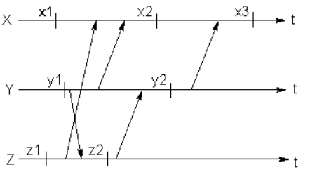
\includegraphics[width=0.24\textwidth]{pics/effect_domino.png}
    
    На рисунке показаны три процесса (X,Y,Z), взаимодействующие через сообщения. Вертикальные черточки показывают на временной оси моменты запоминания состояния процесса для восстановления в случае отказа. Стрелочки соответствуют сообщениям и показывают моменты их отправления и получения. Предположим теперь, что процесс Z сломается и будет восстановлен в состояние z2. Это приведет к откату процесса Y в y1, а затем и процессов X и Z в начальные состояния x1 и y1. Этот эффект известен как эффект домино.
    
    \item Множество контрольных точек называется \textbf{строго консистентным}, если во время его фиксации никаких обменов между процессами не было. 
    Оно соответствует понятию строго консистентного глобального состояния, когда все посланные сообщения получены и нет никаких сообщений в каналах связи.
    \item Множество контрольных точек называется \textbf{консистентным}, если для любой зафиксированной операции приема сообщения, соответствующая операция посылки также зафиксирована (нет сообщений-сирот).
\end{itemize}

\textbf{Методы фиксации контрольных точек}

\begin{enumerate}
    \item \textbf{Простой метод} --- фиксация локальной контрольной точки после каждой операции посылки сообщения. 
    При этом посылка сообщения и фиксация должны быть единой неделимой операцией (транзакцией). 
    Множество последних локальных контрольных точек является консистентным (но не строго консистентным).

    Чтобы избежать потерь сообщений при восстановлении с использованием консистентного множества контрольных точек необходимо повторить отправку тех сообщений, квитанции о получении которых стали недействительными в результате отката. 
    Используя временные метки сообщений можно распознавать сообщения-призраки.
    \item \textbf{Синхронная фиксация.} 
    Два вида контрольных точек - постоянные и пробные. 
    
    \textbf{Постоянная контрольная точка} --- это локальная контрольная точка, являющаяся частью консистентной глобальной контрольной точки. 
    \textit{Пробная контрольная точка} --- это временная контрольная точка, которая становится постоянной только в случае успешного завершения алгоритма.

    \textbf{Фиксация}: \textit{1 фаза}. 
    Инициатор фиксации (процесс $P_i$) создает пробную КТ и просит все остальные процессы сделать то же самое. 
    При этом процессу запрещается посылать неслужебные сообщения после того, как он сделает пробную контрольную точку. 
    Каждый процесс извещает $P_i$ о том, сделал ли он пробную КТ. 
    Если все процессы сделали пробные контрольные точки, то $P_i$ превращает пробные точки в постоянные. 
    Если какой-либо процесс не смог сделать пробную точку, все точки отменяются.

    \textit{2 фаза}. $P_i$ информирует все процессы о своем решении.
    
    \textbf{Восстановление}: \textit{1 фаза}. 
    Инициатор отката спрашивает остальных, готовы ли они откатываться. 
    Когда все будут готовы к откату, откат.

    \textit{2 фаза}. 
    $P_i$ сообщает всем о принятом решении. 
    Получив это сообщение, каждый процесс поступает указанным образом. 
    С момента ответа на опрос готовности и до получения принятого решения процессы не должны посылать сообщения.
    \item \textbf{Асинхронная фиксация.} 
    Множество контрольных точек может быть неконсистентным. 
    При откате происходит поиск подходящего консистентного множества путем поочередного отката каждого процесса в ту точку, в которой зафиксированы все посланные им и полученные другими сообщения.
\end{enumerate}

\textbf{Репликация} - механизм синхронизации содержимого нескольких копий объекта

Рассмотрим возможные протоколы работоспособности коммуникаций и процессоров:

\begin{itemize}
    \item \textit{Протокол принятия единых решений}. 
    
    Все исполнители являются исправными и должны либо все принять, либо все не принять заранее предусмотренное решение.

    \item \textit{Протокол принятия согласованных решений}. 
    
    Наоборот, принятие решения при надежных коммуникациях, но ненадежной работы процессоров. 
    В системе с $m$ неверно работающими процессорами можно достичь согласия только при наличии $2m+1$ верно работающих процессоров (более $2/3$) (задача Византийских генералов).
\end{itemize}

Предположим, что коммуникации надежны, а процессоры нет.

\textit{Алгоритм надежных неделимых широковещательных рассылок сообщений:}
\begin{description}
    \item[\textit{Фаза 1}] Процесс-отправитель посылает сообщение группе процессов (список их идентификаторов содержится в сообщении). 
    Процессы приписывают сообщению приоритет и помещают в очередь (как недоставленное), информируют отправителя.
    \item[\textit{Фаза 2}] Отправитель получил все ответы => выбирает максимальный полученный приоритет и присваивает его сообщению, рассылает всем процессам.
    Получатели принимают, помечают сообщение как доставленное, упорядочивают сообщения в своих очередях.
    \item[] Если получатель обнаружит, что он имеет сообщение с пометкой <недоставленное>, отправитель которого сломался, то он для завершения выполнения протокола осуществляет следующие два шага в качестве координатора: опрашивает всех о статусе сообщения; получив все ответы, реагирует на них. 
    Если сообщение у какого-то получателя помечено как <доставленное>, то его окончательный приоритет рассылается всем. 
    Получив это сообщение каждый процесс выполняет шаги фазы 2. 
    Иначе координатор заново начинает весь протокол с фазы 1.
\end{description}


% -------- source --------
\bigbreak
[\cite{parallel_lec7}]